\chapter{随机变量及其分布}

\begin{definition}{(一维)随机变量}{random variable}
	定义随机变量(random variable)~$X:\Omega\to\RR$是样本空间上的实值函数。有
	\begin{compactitem}
		\item 离散型(discrete):至多可数个取值;
		\item 连续型(continuous):区间型取值(不严格);
		\item 其他
	\end{compactitem}
\end{definition}
\begin{definition}
	{随机变量的概率}{}
	$\forall I\subset\RR$可测,记原像集$X\inv(I)\in\cF$,定义\footnote{这种定义属于好看的鱼(形式简洁),而不属于好吃的鱼(实用)。}
	\[
		\P_X(X\in I):=\P(X\inv(I)),\quad\forall I\subset\RR~\text{可测}
	\]
	一般记$\P_X$为$\P$。
\end{definition}
\begin{definition}{累计分布函数}{cumulative distribution function}
	记$X$的累计分布函数(cumulative distribution function, CDF)\index{CDF, 累计分布函数}
	\[
		\CDF(x):=\P(X\leqslant x),\quad\forall x\in\RR
	\]
	则$\P(a<X\leqslant b)\equiv\CDF(b)-\CDF(a)$。
\end{definition}

\begin{corollary}
	CDF的性质:
	\begin{itemize}
		\item $\CDF(x)$单调递增(不严格单调);
		\item $\lim_{x\to+\infty}\CDF(x)=1,\lim_{x\to-\infty}\CDF(x)=0;$
		\item $\CDF(x)$右连续,不一定左连续。
	\end{itemize}
\end{corollary}
\begin{remark}~
	\begin{compactenum}
		\item 随机要素来自样本点$\omega$的随机选择;
		\item $X,Y$同样本空间时,一般地,$aX+bY$等$X,Y$的函数也是随机变量;
		\item 随机变量同分布$\iff$ CDF相同;但不代表变量相同。
	\end{compactenum}
\end{remark}

\section{离散分布}

\begin{definition}{离散分布}{discrete distribution}
	离散分布可由分布列(probability distribution)表示概率在样本空间中的分布
	\begin{center}
		\begin{tabular}{cccccc}
			\toprule
			$X$&$x_1$&$x_2$&$\cdots$&$x_i$&$\cdots$\\
			\midrule
			$p$&$p_1$&$p_2$&$\cdots$&$p_i$&$\cdots$\\
			\bottomrule
		\end{tabular}
	\end{center}
	% 概率质量函数(probability mass function, PMF)\index{PMF, 概率质量函数}
	% \[
	% 	f(x)=\P(X=x),\quad\forall x\in\RR
	% \]
\end{definition}

\begin{corollary}
	离散分布的CDF为阶梯函数。
\end{corollary}

\begin{definition}{期望和方差}{expectation and variance}
	期望(expectation)即均值
	\begin{equation}
		\E(X):=\sum\nolimits_{i\in I}x_ip_i,
	\end{equation}
	方差(variance)
	\begin{equation}
		\Var(X):=\sum\nolimits_{i\in I}\bigkh{x_i-\E(X)}^2p_i\equiv\E(X^2)-\E(X)^2.
	\end{equation}
\end{definition}

\begin{corollary}
	随机变量$X$的函数$g(X)$的期望
	\[
		\E(g(X))=\sum\nolimits_{i\in I}g(x_i)p_i.
	\]
\end{corollary}

\begin{remark}
	期望存在要求级数绝对收敛。
\end{remark}

\paragraph{二项分布}

~

\begin{definition}{\Bern 分布}{Bernoulli distribution}
	\Bern 分布也称0-1分布,$p$为成功概率,记作$X\sim\Bino(p)$,其分布列为
	\begin{equation}
		\P(X=k)=\begin{cases}
			1-p,&k=0\\
			p,&k=1
		\end{cases}
	\end{equation}
	% \begin{center}
	% 	\begin{tabular}{ccc}
	% 		\toprule
	% 		$X$&0&1\\
	% 		\midrule
	% 		$p$&$1-p$&$p$\\
	% 		\bottomrule
	% 	\end{tabular}
	% \end{center}
\end{definition}

\begin{definition}{二项分布}{binominal distribution}
	$n$次独立\Bern 试验的成功次数$X$服从二项分布(binominal distribution),记作$X\sim\Bino(n,p)$,
	\begin{equation}
		\P(X=k)=\binom nk p^k(1-p)^{n-k},\quad k=0,\ldots,n
	\end{equation}
	\begin{center}
		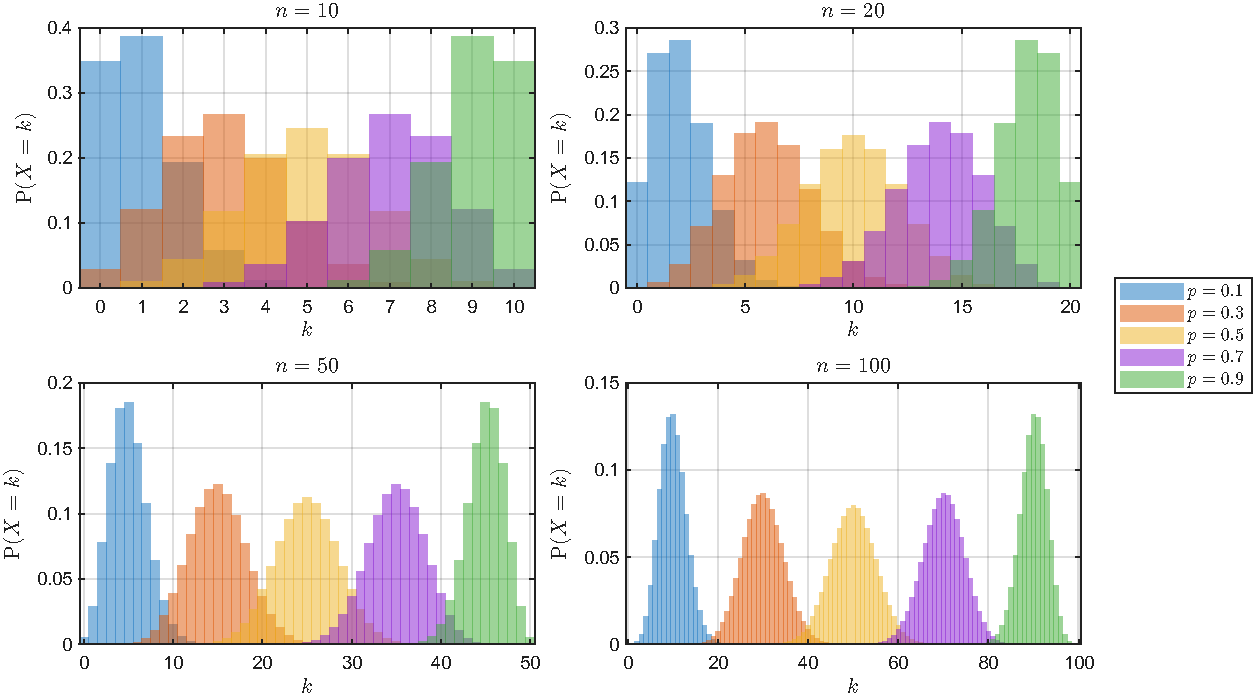
\includegraphics[width=.95\textwidth]{figures/pdf_bin.pdf}
		\captionof{figure}{不同$n,p$下的二项分布}
	\end{center}
\end{definition}

\begin{corollary}
	% 显然\Bern 分布就是二项分布的特例。
	二项分布的期望和方差为
	\begin{subequations}
		\begin{align}
			\E(X)&=np,\\
			\Var(X)&=np(1-p).
		\end{align}
	\end{subequations}
\end{corollary}

\paragraph{Poisson分布}

我们考虑一个时间段内的事件次数$X\sim\Bino(n,p)$,其中$n$是时间段的切片份数。
保持其期望$\E(X)=np=:\lambda$不变,令$n\to\infty$,即事件可能发生在任一时刻,则
\[
	\lim_{n\to\infty}\binom nk\kh{\frac\lambda{n}}^k\kh{1-\frac\lambda{n}}^{n-k}=\lim_{n\to\infty}\frac{\lambda^k}{k!}\kh{1-\frac\lambda{n}}^n\cancel{\frac{n!}{n^k(n-k)!}}\cancel{\kh{1-\frac\lambda{n}}^{-k}}=\frac{\lambda^k}{k!}\e{-\lambda}.
\]
% 我们便得到了一个新的分布,称为Poisson分布。

\begin{definition}{Poisson分布}{Poisson distribution}
	小概率事件在一段时间内发生的次数$X$服从Poisson分布,记作$X\sim\Pois(\lambda)$,
	\[
		\P(X=k)=\frac{\lambda^k}{k!}\e{-\lambda},\quad k=0,1,2,\ldots
	\]
	\begin{center}
		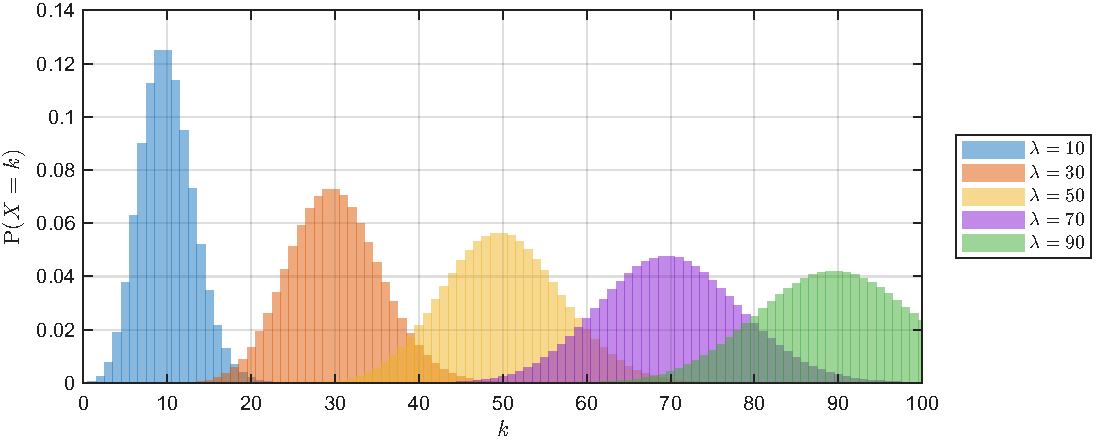
\includegraphics[width=.9\textwidth]{figures/pdf_poission.pdf}
		\captionof{figure}{不同$\lambda$下的Poisson分布}
	\end{center}
\end{definition}
\begin{corollary}
	Poisson分布的期望和方差为
	\begin{subequations}
		\begin{align}
			\E(X)&=\lambda,\\
			\Var(X)&=\lambda.
		\end{align}
	\end{subequations}
\end{corollary}

\begin{theorem}{Poisson分布近似二项分布}{}
	用$\Pois(np)$近似$\Bino(n,p)$的误差最多为$\min(p,np^2)$。
\end{theorem}

\begin{remark}
	若试验不独立,但满足弱相依条件下,Poisson分布仍为较好近似。
\end{remark}

\begin{example}{弱相依条件举例:配对问题}{weak dependence condition}
	在\exmref{exm:derangement} 中,尽管$A_i$和$A_j$并不独立,但弱相依
	\[
		\P(A_i)=\frac1n\approx\P(A_i|A_j)=\frac1{n-1}.
	\]
	记$X=$拿到自己帽子的人数,当$n\to\infty$时,$X\sim\Pois(1)$
	\[
		\P(X=k)=\frac{\e{-1}}{k!},\quad k=0,1,2,\ldots
	\]
	\tcblower
	下面用常规做法检验:指定$k$个人,记
	\begin{itemize}
		\item $E=$这$k$个人都拿到自己的帽子;
		\item $F=$余下$n-k$个人都未拿到自己的帽子。
	\end{itemize}
	则$\P(F|E)$就是$n-k$个人的错排问题,根据\exmref{exm:derangement} 中的结果:
	\[
		\P(E\cap F)=\P(E)\P(F|E)=\frac{(n-k)!}{n!}\cdot\frac{!(n-k)}{(n-k)!},
	\]
	对于$\P(X=k)$来说,由于这$k$个人是任选的,故
	\[
		\P(X=k)=\binom nk\P(E\cap F)=\frac1{k!}\cdot\frac{!(n-k)}{(n-k)!}\to\frac{1}{k!}\cdot\frac1{\e{}}.
	\]
\end{example}

\section{连续分布}

\begin{definition}{连续分布}{continuous distribution}
	若存在$f(x)\geqslant 0$,使得$\forall I\subset\RR$可测,都有
	\[
		\P(X\in I)=\int_If(x)\d x
	\]
	则称$X$为连续型随机变量,服从连续分布,$f(x)$为概率密度函数(probability density function, PDF)。\index{PDF, 概率密度函数}
\end{definition}

\begin{corollary}
	连续分布的性质:
	\begin{itemize}
		\item $\forall x\in\RR,\enspace\P(X=x)\equiv 0;$
		\item 归一性:
			\begin{equation}
				\int\iti f(x)\d x\equiv 1;
			\end{equation}
		\item 期望和方差(要求积分\textbf{绝对收敛})
			\begin{subequations}
				\begin{align}
					\E(X)&=\int\iti xf(x)\d x,\\
					\Var(X)&=\int\iti(x-\E(X))^2f(x)\d x.
				\end{align}
			\end{subequations}
		\item 连续分布的CDF $\CDF(x)$连续且可导,且
			\begin{equation}
				\CDF'(x)=f(x).
			\end{equation}
			若$\CDF(x)$严格递增,则$\CDF^{-1}(y)$存在;但若其不严格递增,也可well define
			\begin{equation}
				\label{eq:CDF-1}
				\CDF^{-1}(y):=\inf\set x{\CDF(x)\geqslant y}.
			\end{equation}
	\end{itemize}
\end{corollary}
\iffalse
\begin{example}{常见连续分布}{}
	\begin{compactenum}
		\item 均匀分布$f(x;a,b)=\frac1{b-a},a\leqslant x\leqslant b;$
		\item 指数分布$f(x;\lambda)=\lambda\e{-\lambda x},x\geqslant 0;$
		\item 正态分布$f(x;\mu,\sigma^2)=\frac1{\sqrt{2\pi}\sigma}\e{-(x-\mu)^2/2\sigma^2},-\infty<x<\infty;$
		\item 伽玛分布$f(x;\alpha,\lambda)=\frac{\lambda^\alpha}{\Gamma(\alpha)}x^{\alpha-1}\e{-\lambda x}.x\geqslant 0;$
		\item 卡方分布$f(x;n)=\frac{x^{n/2-1}}{2^{n/2}\Gamma(n/2)}\e{-x/2},x\geqslant 0;$
	\end{compactenum}
\end{example}
\fi
\begin{definition}{均匀分布}{uniform distribution}
	均匀分布(uniform distribution)记作$X\sim\Unif(a,b)$,%随机数$\Unif(0,1)$
	\begin{equation}
		f(x)=\begin{cases}
			\frac1{b-a},&x\in(a,b)\\
			0,&\text{elsewhere}
		\end{cases}
	\end{equation}
	特别地,服从标准均匀分布的随机变量$X\sim\Unif(0,1)$也称为随机数。
\end{definition}
\begin{corollary}
	均匀分布的期望和方差为
	\begin{subequations}
		\begin{align}
			\E(X)&=\frac{a+b}2,\\
			\Var(X)&=\frac{(b-a)^2}{12}.
		\end{align}
	\end{subequations}
\end{corollary}
\begin{definition}{正态分布}{normal distribution}
	正态分布(normal distribution)记作$X\sim\Norm(\mu,\sigma^2)$,%标准正态$\Norm(0,1)$
	\begin{equation}
		f(x)=\frac1{\sqrt{2\pi}\sigma}\exp\biggfkh{-\frac{(x-\mu)^2}{2\sigma^2}},\quad x\in\RR
	\end{equation}
	特别地,标准正态分布$\Norm(0,1)$的CDF记作$\Phi(x)$。
	\begin{center}
		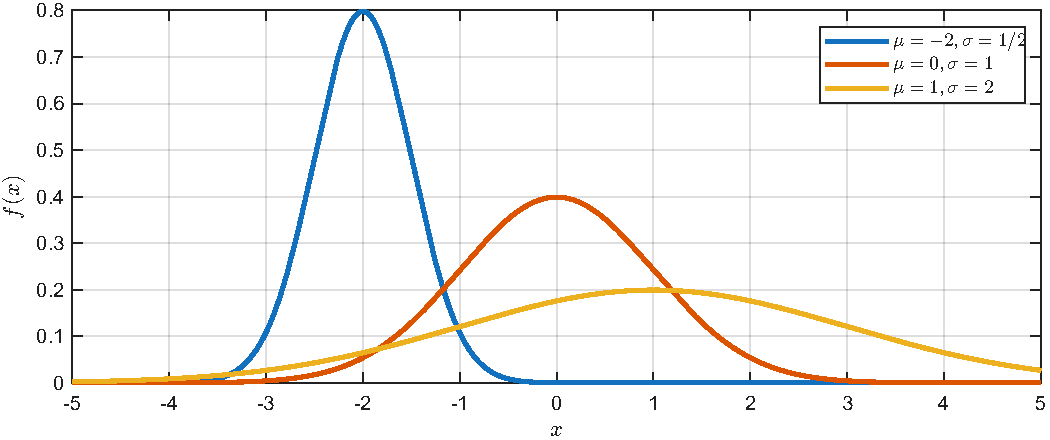
\includegraphics[width=.9\textwidth]{figures/pdf_normal.pdf}
		\captionof{figure}{不同$\mu,\sigma$下的正态分布}
	\end{center}
\end{definition}
\begin{corollary}
	正态分布的期望和方差为
	\begin{subequations}
		\begin{align}
			\E(X)&=\mu,\\
			\Var(X)&=\sigma^2.
		\end{align}
	\end{subequations}
\end{corollary}
\begin{definition}{指数分布}{exponential distribution}
	指数分布(exponential distribution)通常刻画寿命、等待时间,记作$X\sim\Expo(\lambda)$,
	\begin{equation}
		f(x)=\begin{cases}
			\lambda\e{-\lambda x},&x>0\\
			0,&x\leqslant 0
		\end{cases}
	\end{equation}
	\begin{center}
		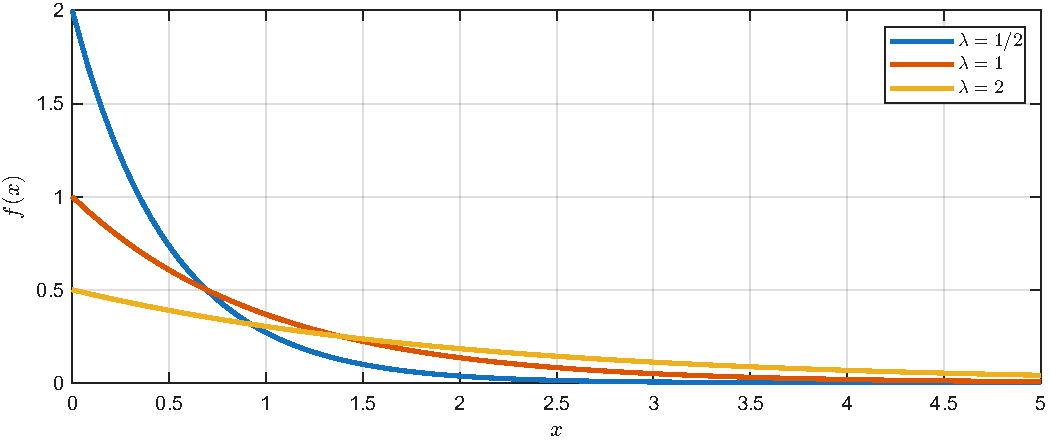
\includegraphics[width=.9\textwidth]{figures/pdf_exp.pdf}
		\captionof{figure}{不同$\lambda$下的指数分布}
	\end{center}
\end{definition}

\begin{corollary}
	指数分布的期望和方差为
	\begin{subequations}
		\begin{align}
			\E(X)&=\frac1\lambda,\\
			\Var(X)&=\frac1{\lambda^2}.
		\end{align}
	\end{subequations}
	其期望往往被定义为平均寿命$\beta:=\E(X)\equiv 1/\lambda$,因此也有教材将指数分布记作$\Expo(\beta)$。
\end{corollary}

\begin{corollary}
	指数分布的尾概率与Poisson分布有关:
	\[
		\P_{\Expo(\lambda)}(T>\tau)=\e{-\lambda\tau}=\P_{\Pois(\lambda\tau)}(N=0).
	\]
	这说明:如果时间$(0,\tau)$内事件的发生次数$N\sim\Pois(\lambda\tau)$,则相邻事件的时间间隔$\D T\sim\Expo(\lambda)$。
\end{corollary}

\begin{example}{指数分布的导出}{}
	产品在$(x,x+\d x)$时间内的失效率为
	\[
		\P(x<X<x+\d x|X>x)=\frac{\P(x<X<x+\d x)}{\P(X>x)}=\frac{\CDF(x+\d x)-\CDF(x)}{1-\CDF(x)}=\frac{\CDF'(x)}{1-\CDF(x)}\d x
	\]
	令失效率为$\lambda(x)\d x$
	\[
		\frac{\CDF'(x)}{1-\CDF(x)}=\lambda(x),\implies\CDF(x)=1-\exp\biggfkh{-\int_0^x\lambda(t)\d t}.
	\]
	若假设无老化:$\lambda(t)\equiv\lambda$,则分布为指数分布:
	\begin{equation}
		\CDF(x)=1-\e{-\lambda x},\quad x>0,
	\end{equation}

	这体现出指数分布的无记忆性:$\forall\tau>0$
	\[
		\P(X>t+\tau|X>\tau)=\frac{\e{-\lambda(t+\tau)}}{\e{-\lambda\tau}}=\e{-\lambda t}=\P(X>t)
	\]

	\tcblower
	
	改进$\lambda(x)=\alpha x^{\alpha+1}/\beta^\alpha$,得到Weibull分布
	\begin{equation}
		\label{eq:Weibull CDF}
		\CDF(x)=1-\e{-(x/\beta)^\alpha},\quad x>0.
	\end{equation}
\end{example}

\section{随机变量的函数}

\begin{theorem}
	{离散型随机变量的函数}{}
	$X$离散$\implies Y:=g(X)$离散。
\end{theorem}

\begin{theorem}{连续型随机变量的函数}{}
	若$g$处处可导且严格单调,则$Y=g(X)$的PDF为
	\begin{equation}
		f_Y(y)=f_X\bigkh{g^{-1}(y)}\abs{\fkh{g^{-1}(y)}'}.
	\end{equation}
	其本质是
	\begin{equation}
		\CDF_Y(y)=\CDF_X\bigkh{g^{-1}(y)}.
	\end{equation}
\end{theorem}
\begin{example}{生成随机变量}{}
	服从CDF $\CDF(y)$的随机变量$Y$可由随机数$X\sim\Unif(0,1)$生成:
	\begin{equation}
		Y=\CDF\inv(X).
	\end{equation}
\end{example}
\section*{Review}
\begin{compactenum}
	\item PMF/PDF, CDF
	\item 期望$\mu$、标准差$\sigma$;标准化$\frac{X-\mu}\sigma$
	\item 参数的意义:位置、尺度、形状
	\item $Y=g(X)$
\end{compactenum}